\documentclass[tikz]{standalone}

\def\rA{3cm}
\def\rB{1.1 * \rA}
\def\s{1mm}

\begin{document}
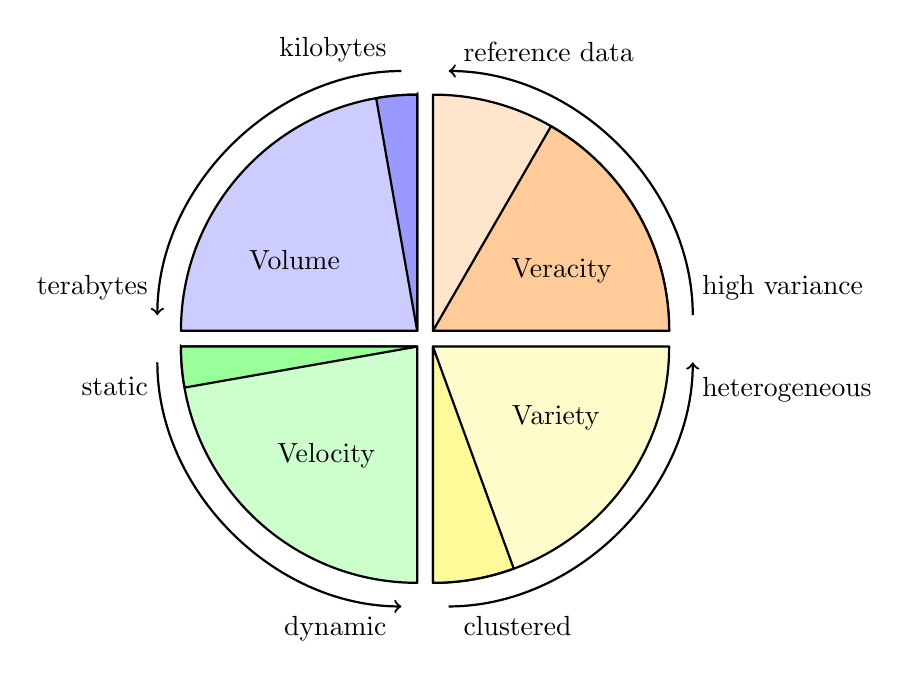
\begin{tikzpicture}[
    thick, every path/.style={rounded corners=0.1},
    direction/.style={->,shorten >=2mm,shorten <=2mm},
  ]

  \begin{scope}[shift={(\s,\s)}]
    \draw [fill=orange!20] (0:\rA) arc(0:90:\rA) |- cycle;
    \draw [fill=orange!40] (0:\rA) arc(0:60:\rA) -- (0,0) -- cycle;
    \node at (25:0.6*\rA) {Veracity};
    \draw[direction] (0:\rB) arc(0:90:\rB) node[pos=0.05, above right] {high variance} node[pos=0.95, above right] {reference data};
  \end{scope}

  \begin{scope}[shift={(-\s,\s)}]
    \draw [fill=blue!20] (90:\rA) arc(90:180:\rA) -| cycle;
    \draw [fill=blue!40] (90:\rA) arc(90:100:\rA) -- (0,0) -- cycle;
    \node at (150:0.6*\rA) {Volume};
    \draw[direction] (90:\rB) arc(90:180:\rB) node[pos=0.05, above left] {kilobytes} node[pos=0.95, above left] {terabytes};
  \end{scope}

  \begin{scope}[shift={(-\s,-\s)}]
    \draw [fill=green!20] (180:\rA) arc(180:270:\rA) |- cycle;
    \draw [fill=green!40] (180:\rA) arc(180:190:\rA) -- (0,0) -- cycle;
    \node at (230:0.6*\rA) {Velocity};
    \draw[direction] (180:\rB) arc(-180:-90:\rB) node[pos=0.05, below left] {static} node[pos=0.95, below left] {dynamic};
  \end{scope}

  \begin{scope}[shift={(\s,-\s)}]
    \draw [fill=yellow!20] (270:\rA) arc(270:360:\rA) -| cycle;
    \draw [fill=yellow!40] (270:\rA) arc(270:290:\rA) -- (0,0) -- cycle;
    \node at (330:0.6*\rA) {Variety};
    \draw[direction] (270:\rB) arc(-90:0:\rB) node[pos=0.05, below right] {clustered} node[pos=0.95, below right] {heterogeneous};
  \end{scope}

\end{tikzpicture}
\end{document}
